\chapter{Geometria analitica y lugares geometricos}

\begin{theorybox}{Trazabilidad del capitulo}
Este capitulo desarrolla las secciones \texttt{C07.S01-C07.S10} de la matriz de cobertura a
partir de \texttt{sources/Relacion ejercicios temas 6 y 7.pdf}. La progresion parte de la recta
como objeto algebraico y termina en construcciones geometricas y problemas de compatibilidad.
\end{theorybox}

\section{[C07.S01] Ecuaciones de la recta y vectores asociados}

\subsection*{Objetivos de aprendizaje}
\begin{itemize}
  \item Hallar ecuaciones de rectas a partir de puntos y direcciones.
  \item Reconocer vectores director y normal de una recta.
\end{itemize}

\subsection*{Prerrequisitos}
\begin{itemize}
  \item Pendiente de una recta y operaciones con vectores.
\end{itemize}

\begin{theorybox}{Idea minima}
Una recta puede escribirse de varias formas. Si conoces un punto \(P(x_0,y_0)\) y un vector
director \(v=(a,b)\), una forma util es
\[
(x,y)=(x_0,y_0)+t(a,b).
\]
Si conoces un vector normal \(n=(A,B)\), la forma general es
\[
Ax+By+C=0.
\]
\end{theorybox}

\begin{methodbox}{Como reconocer y resolver}
\begin{enumerate}
  \item Si tienes dos puntos, construye un vector director restando coordenadas.
  \item Si tienes una ecuacion general, el vector normal sale de sus coeficientes.
  \item Cambia de forma solo cuando te ayude a responder lo que piden.
\end{enumerate}
\end{methodbox}

\begin{solvedexample}{[EX-C07.S01-01] De dos puntos a la recta}
Halla la ecuacion de la recta que pasa por \(A(1,2)\) y \(B(4,5)\). Indica tambien un vector
director y un vector normal.

\textbf{Desarrollo.} Un vector director es
\[
\overrightarrow{AB}=(4-1,5-2)=(3,3).
\]
Podemos simplificarlo a \((1,1)\). La pendiente vale \(1\), asi que la recta tiene forma
\[
y=x+b.
\]
Usando el punto \(A(1,2)\):
\[
2=1+b \Longrightarrow b=1.
\]
Luego
\[
y=x+1.
\]
Pasando a forma general:
\[
x-y+1=0.
\]
De aqui sale un vector normal, por ejemplo \((1,-1)\).

\textbf{Respuesta final.}
\[
r:\ y=x+1,
\qquad
v_d=(1,1),
\qquad
v_n=(1,-1).
\]
\end{solvedexample}

\begin{commonerror}{Tomar como director el vector normal}
En \(Ax+By+C=0\), el vector \((A,B)\) es normal, no director. El director debe ser
perpendicular a ese vector.
\end{commonerror}

\begin{guidedexercise}{[GX-C07.S01-01] Punto y direccion}
Halla la ecuacion de la recta que pasa por \((0,2)\) y tiene vector director \((1,-1)\).

\textbf{Pista 1.} Su pendiente es \(-1\).
\end{guidedexercise}

\begin{shortanswer}{[GX-C07.S01-01]}
\[
y=-x+2.
\]
\end{shortanswer}

\begin{fullsolution}{[GX-C07.S01-01]}
Con pendiente \(-1\), la recta es \(y=-x+b\). Como pasa por \((0,2)\), se tiene \(b=2\).
\end{fullsolution}

\begin{guidedexercise}{[GX-C07.S01-02] Director y normal desde la forma general}
Para la recta \(2x-3y+6=0\), indica un vector director y un vector normal.

\textbf{Pista 1.} El normal sale directamente de la ecuacion.
\end{guidedexercise}

\begin{shortanswer}{[GX-C07.S01-02]}
Vector normal: \((2,-3)\). Vector director: \((3,2)\).
\end{shortanswer}

\begin{fullsolution}{[GX-C07.S01-02]}
El vector normal es \((2,-3)\). Un vector perpendicular a el es \((3,2)\), que sirve como
director.
\end{fullsolution}

\subsection*{Practica autonoma graduada}
\begin{exercise}{[PX-C07.S01-01] Halla la ecuacion de la recta que pasa por \((2,1)\) y \((2,5)\).}
\end{exercise}
\begin{exercise}{[PX-C07.S01-02] Halla la ecuacion de la recta que pasa por \((0,-1)\) y tiene pendiente \(3\).}
\end{exercise}
\begin{exercise}{[PX-C07.S01-03] Halla la ecuacion de la recta que pasa por \((1,4)\) y \((3,0)\).}
\end{exercise}
\begin{exercise}{[PX-C07.S01-04] Indica un vector normal de la recta \(x-2y+5=0\).}
\end{exercise}
\begin{exercise}{[PX-C07.S01-05] Indica un vector director de la recta \(3x+y-7=0\).}
\end{exercise}
\begin{exercise}{[PX-C07.S01-06] Halla la recta que pasa por \((-1,2)\) y es paralela a \(x+y=4\).}
\end{exercise}

\begin{shortanswer}{C07.S01 practica autonoma}
\begin{enumerate}[label=\textbf{PX-C07.S01-\arabic*:}, leftmargin=*]
  \item \(x=2\)
  \item \(y=3x-1\)
  \item \(y=-2x+6\)
  \item \((1,-2)\)
  \item \((1,-3)\)
  \item \(y=-x+1\)
\end{enumerate}
\end{shortanswer}

\begin{fullsolution}{C07.S01 practica autonoma}
\begin{enumerate}[label=\textbf{PX-C07.S01-\arabic*:}, leftmargin=*]
  \item Es una recta vertical, luego \(x=2\).
  \item Con pendiente \(3\) y paso por \((0,-1)\), sale \(y=3x-1\).
  \item La pendiente es \(\frac{0-4}{3-1}=-2\), asi que \(y=-2x+6\).
  \item De la forma general, el vector normal es \((1,-2)\).
  \item Un director perpendicular a \((3,1)\) es \((1,-3)\).
  \item La recta \(x+y=4\) tiene pendiente \(-1\). Pasando por \((-1,2)\), queda \(y=-x+1\).
\end{enumerate}
\end{fullsolution}

\section{[C07.S02] Problemas con parametros en rectas}

\subsection*{Objetivos de aprendizaje}
\begin{itemize}
  \item Determinar parametros para que una recta cumpla una condicion.
  \item Relacionar paso por punto, pendiente y paralelismo.
\end{itemize}

\subsection*{Prerrequisitos}
\begin{itemize}
  \item Ecuaciones de la recta y sistemas lineales.
\end{itemize}

\begin{theorybox}{Idea minima}
Un parametro en la ecuacion de una recta se fija imponiendo una condicion concreta: que la
recta pase por un punto, sea paralela, perpendicular o tenga un cierto corte.
\end{theorybox}

\begin{methodbox}{Como reconocer y resolver}
\begin{enumerate}
  \item Traduce la condicion geometricamente.
  \item Sustituye el punto o iguala pendientes segun corresponda.
  \item Resuelve la ecuacion del parametro.
\end{enumerate}
\end{methodbox}

\begin{solvedexample}{[EX-C07.S02-01] Parametro por paso por punto}
Determina \(a\) para que la recta
\[
(a-1)x+2y=5
\]
pase por el punto \((1,2)\).

\textbf{Desarrollo.} Sustituimos las coordenadas del punto:
\[
(a-1)\cdot 1+2\cdot 2=5.
\]
Entonces
\[
a-1+4=5 \Longrightarrow a=2.
\]

\textbf{Respuesta final.}
\[
a=2.
\]
\end{solvedexample}

\begin{commonerror}{Olvidar sustituir las dos coordenadas}
Para comprobar si un punto pertenece a una recta, hay que sustituir \(x\) y \(y\). Si se usa
solo una coordenada, la condicion queda incompleta.
\end{commonerror}

\begin{guidedexercise}{[GX-C07.S02-01] Paralelismo}
Halla \(k\) para que \(y=(k+1)x-3\) sea paralela a \(2x-y+1=0\).

\textbf{Pista 1.} Pasa la segunda recta a forma explicita.
\end{guidedexercise}

\begin{shortanswer}{[GX-C07.S02-01]}
\[
k=1.
\]
\end{shortanswer}

\begin{fullsolution}{[GX-C07.S02-01]}
La recta \(2x-y+1=0\) se escribe \(y=2x+1\), asi que su pendiente es \(2\). Para que las
rectas sean paralelas:
\[
k+1=2 \Longrightarrow k=1.
\]
\end{fullsolution}

\begin{guidedexercise}{[GX-C07.S02-02] Perpendicularidad}
Halla \(k\) para que \(x+ky=4\) sea perpendicular a \(y=x\).

\textbf{Pista 1.} La pendiente de \(y=x\) es \(1\).
\end{guidedexercise}

\begin{shortanswer}{[GX-C07.S02-02]}
\[
k=1.
\]
\end{shortanswer}

\begin{fullsolution}{[GX-C07.S02-02]}
La recta \(x+ky=4\) se escribe
\[
y=-\frac{1}{k}x+\frac{4}{k}.
\]
Para que sea perpendicular a una recta de pendiente \(1\), debe tener pendiente \(-1\):
\[
-\frac{1}{k}=-1 \Longrightarrow k=1.
\]
\end{fullsolution}

\subsection*{Practica autonoma graduada}
\begin{exercise}{[PX-C07.S02-01] Halla \(m\) para que \(2x+(m-1)y=5\) pase por \((1,1)\).}
\end{exercise}
\begin{exercise}{[PX-C07.S02-02] Halla \(k\) para que \(y=(2k-1)x+4\) sea paralela a \(y=3x-2\).}
\end{exercise}
\begin{exercise}{[PX-C07.S02-03] Halla \(a\) para que \(ax-y+2=0\) sea perpendicular a \(y=2x+1\).}
\end{exercise}
\begin{exercise}{[PX-C07.S02-04] Halla \(b\) para que \(x+by-6=0\) pase por \((2,4)\).}
\end{exercise}
\begin{exercise}{[PX-C07.S02-05] Halla \(c\) para que \((c+1)x+2y=0\) sea paralela a \(x-2y+3=0\).}
\end{exercise}
\begin{exercise}{[PX-C07.S02-06] Halla \(d\) para que \(x-dy+1=0\) sea perpendicular a \(y=-x\).}
\end{exercise}

\begin{shortanswer}{C07.S02 practica autonoma}
\begin{enumerate}[label=\textbf{PX-C07.S02-\arabic*:}, leftmargin=*]
  \item \(m=4\)
  \item \(k=2\)
  \item \(a=-\frac{1}{2}\)
  \item \(b=1\)
  \item \(c=-2\)
  \item \(d=1\)
\end{enumerate}
\end{shortanswer}

\begin{fullsolution}{C07.S02 practica autonoma}
\begin{enumerate}[label=\textbf{PX-C07.S02-\arabic*:}, leftmargin=*]
  \item \(2+(m-1)=5\), luego \(m=4\).
  \item Para que sea paralela a pendiente \(3\): \(2k-1=3\), de donde \(k=2\).
  \item La recta es \(y=ax+2\). Su pendiente debe ser \(-\frac{1}{2}\).
  \item \(2+4b-6=0\), luego \(b=1\).
  \item La recta dada tiene pendiente \(\frac{1}{2}\). Como la nuestra tiene pendiente
  \(-\frac{c+1}{2}\), sale \(c=-2\).
  \item La recta \(y=-x\) tiene pendiente \(-1\), asi que la perpendicular debe tener pendiente
  \(1\). En \(x-dy+1=0\), la pendiente es \(\frac{1}{d}\), luego \(d=1\).
\end{enumerate}
\end{fullsolution}

\section{[C07.S03] Simetrias respecto de punto y recta}

\subsection*{Objetivos de aprendizaje}
\begin{itemize}
  \item Hallar puntos simetricos respecto de un centro o de una recta sencilla.
  \item Interpretar una simetria como una conservacion de distancias.
\end{itemize}

\subsection*{Prerrequisitos}
\begin{itemize}
  \item Coordenadas y punto medio.
\end{itemize}

\begin{theorybox}{Idea minima}
Si \(P'\) es el simetrico de \(P\) respecto de un punto \(C\), entonces \(C\) es el punto medio
del segmento \(PP'\). En simetrias respecto de rectas sencillas, se conserva una coordenada y
se refleja la otra.
\end{theorybox}

\begin{methodbox}{Como reconocer y resolver}
\begin{enumerate}
  \item Para simetria central, usa la formula del punto medio.
  \item Para rectas verticales u horizontales, refleja solo la coordenada perpendicular.
  \item Comprueba al final que las distancias a la recta o al centro son iguales.
\end{enumerate}
\end{methodbox}

\begin{solvedexample}{[EX-C07.S03-01] Simetria central}
Halla el simetrico de \(P(3,1)\) respecto del punto \(C(1,2)\).

\textbf{Desarrollo.} Si \(P'(x,y)\) es el simetrico, \(C\) es el punto medio de \(PP'\), luego
\[
\frac{3+x}{2}=1,
\qquad
\frac{1+y}{2}=2.
\]
De aqui,
\[
x=-1,
\qquad
y=3.
\]

\textbf{Respuesta final.}
\[
P'(-1,3).
\]
\end{solvedexample}

\begin{commonerror}{Intercambiar punto medio y extremo}
La simetria central no consiste en copiar las coordenadas del centro. El centro queda justo en
medio del segmento que une punto original y punto simetrico.
\end{commonerror}

\begin{guidedexercise}{[GX-C07.S03-01] Simetria respecto del eje \(X\)}
Halla el simetrico de \(A(4,-2)\) respecto del eje \(X\).
\end{guidedexercise}

\begin{shortanswer}{[GX-C07.S03-01]}
\[
A'(4,2).
\]
\end{shortanswer}

\begin{fullsolution}{[GX-C07.S03-01]}
Se conserva la coordenada \(x\) y cambia de signo la coordenada \(y\):
\[
A'(4,2).
\]
\end{fullsolution}

\begin{guidedexercise}{[GX-C07.S03-02] Simetria respecto de una recta vertical}
Halla el simetrico de \(B(1,5)\) respecto de la recta \(x=2\).

\textbf{Pista 1.} La recta \(x=2\) debe quedar a la misma distancia de \(B\) y de su simetrico.
\end{guidedexercise}

\begin{shortanswer}{[GX-C07.S03-02]}
\[
B'(3,5).
\]
\end{shortanswer}

\begin{fullsolution}{[GX-C07.S03-02]}
El punto \(B\) esta a distancia \(1\) de la recta \(x=2\). El simetrico queda a distancia \(1\)
al otro lado, con la misma ordenada:
\[
B'(3,5).
\]
\end{fullsolution}

\subsection*{Practica autonoma graduada}
\begin{exercise}{[PX-C07.S03-01] Halla el simetrico de \((2,-1)\) respecto del origen.}
\end{exercise}
\begin{exercise}{[PX-C07.S03-02] Halla el simetrico de \((-3,4)\) respecto del eje \(Y\).}
\end{exercise}
\begin{exercise}{[PX-C07.S03-03] Halla el simetrico de \((5,1)\) respecto de la recta \(x=1\).}
\end{exercise}
\begin{exercise}{[PX-C07.S03-04] Halla el simetrico de \((2,5)\) respecto de la recta \(y=1\).}
\end{exercise}
\begin{exercise}{[PX-C07.S03-05] Halla el simetrico de \(P(4,0)\) respecto de \(M(1,-2)\).}
\end{exercise}
\begin{exercise}{[PX-C07.S03-06] Halla el simetrico de \((3,1)\) respecto de la recta \(y=x\).}
\end{exercise}

\begin{shortanswer}{C07.S03 practica autonoma}
\begin{enumerate}[label=\textbf{PX-C07.S03-\arabic*:}, leftmargin=*]
  \item \((-2,1)\)
  \item \((3,4)\)
  \item \((-3,1)\)
  \item \((2,-3)\)
  \item \((-2,-4)\)
  \item \((1,3)\)
\end{enumerate}
\end{shortanswer}

\begin{fullsolution}{C07.S03 practica autonoma}
\begin{enumerate}[label=\textbf{PX-C07.S03-\arabic*:}, leftmargin=*]
  \item Respecto del origen cambian de signo ambas coordenadas.
  \item Respecto del eje \(Y\), cambia el signo de \(x\).
  \item La recta \(x=1\) queda como punto medio entre \(x=5\) y \(x'=-3\).
  \item Respecto de \(y=1\), la distancia vertical es \(4\), luego \(y'=-3\).
  \item
  \[
  \frac{4+x}{2}=1,\qquad \frac{0+y}{2}=-2,
  \]
  de donde \(x=-2\), \(y=-4\).
  \item En la recta \(y=x\) se intercambian las coordenadas.
\end{enumerate}
\end{fullsolution}

\section{[C07.S04] Posicion relativa de rectas}

\subsection*{Objetivos de aprendizaje}
\begin{itemize}
  \item Clasificar dos rectas como secantes, paralelas o coincidentes.
  \item Hallar puntos de interseccion cuando existan.
\end{itemize}

\subsection*{Prerrequisitos}
\begin{itemize}
  \item Ecuaciones de la recta y resolucion de sistemas \(2\times 2\).
\end{itemize}

\begin{theorybox}{Idea minima}
Dos rectas:
\begin{itemize}
  \item son secantes si tienen pendientes distintas;
  \item son paralelas si tienen la misma pendiente y distinto termino independiente;
  \item son coincidentes si representan la misma ecuacion.
\end{itemize}
\end{theorybox}

\begin{methodbox}{Como reconocer y resolver}
\begin{enumerate}
  \item Lleva las rectas a una forma comparable.
  \item Compara pendientes o coeficientes.
  \item Si son secantes, resuelve el sistema para hallar el punto de corte.
\end{enumerate}
\end{methodbox}

\begin{solvedexample}{[EX-C07.S04-01] Rectas secantes}
Estudia la posicion relativa de las rectas
\[
r:\ x+y=3,
\qquad
s:\ x-y=1.
\]

\textbf{Desarrollo.} Como las pendientes son \(-1\) y \(1\), las rectas son secantes.
Buscamos su punto de corte resolviendo
\[
\begin{cases}
x+y=3,\\
x-y=1.
\end{cases}
\]
Sumando ambas ecuaciones:
\[
2x=4 \Longrightarrow x=2.
\]
Entonces
\[
y=1.
\]

\textbf{Respuesta final.}
\[
r \text{ y } s \text{ son secantes en } (2,1).
\]
\end{solvedexample}

\begin{commonerror}{Confundir paralelas con coincidentes}
Que dos rectas tengan la misma pendiente no basta para que coincidan. Tambien deben compartir
todos sus puntos.
\end{commonerror}

\begin{guidedexercise}{[GX-C07.S04-01] Paralelas}
Estudia la posicion relativa de \(x+2y=1\) y \(x+2y=5\).
\end{guidedexercise}

\begin{shortanswer}{[GX-C07.S04-01]}
Son paralelas.
\end{shortanswer}

\begin{fullsolution}{[GX-C07.S04-01]}
Tienen exactamente los mismos coeficientes en \(x\) e \(y\), pero distinto termino
independiente. Por tanto, son paralelas distintas.
\end{fullsolution}

\begin{guidedexercise}{[GX-C07.S04-02] Coincidentes}
Estudia la posicion relativa de \(2x-y=4\) y \(4x-2y=8\).
\end{guidedexercise}

\begin{shortanswer}{[GX-C07.S04-02]}
Son coincidentes.
\end{shortanswer}

\begin{fullsolution}{[GX-C07.S04-02]}
La segunda ecuacion es el doble de la primera, asi que describen la misma recta.
\end{fullsolution}

\subsection*{Practica autonoma graduada}
\begin{exercise}{[PX-C07.S04-01] Estudia la posicion relativa de \(y=2x+1\) y \(y=-x+4\).}
\end{exercise}
\begin{exercise}{[PX-C07.S04-02] Estudia la posicion relativa de \(x-3y=2\) y \(2x-6y=5\).}
\end{exercise}
\begin{exercise}{[PX-C07.S04-03] Estudia la posicion relativa de \(x+y=0\) y \(3x+3y=0\).}
\end{exercise}
\begin{exercise}{[PX-C07.S04-04] Estudia la posicion relativa de \(x=2\) y \(y=3\).}
\end{exercise}
\begin{exercise}{[PX-C07.S04-05] Estudia la posicion relativa de \(y=-2x+5\) y \(2y=-4x+1\).}
\end{exercise}
\begin{exercise}{[PX-C07.S04-06] Estudia la posicion relativa de \(x-y=1\) y \(x+y=5\).}
\end{exercise}

\begin{shortanswer}{C07.S04 practica autonoma}
\begin{enumerate}[label=\textbf{PX-C07.S04-\arabic*:}, leftmargin=*]
  \item Secantes en \((1,3)\)
  \item Paralelas
  \item Coincidentes
  \item Secantes en \((2,3)\)
  \item Paralelas
  \item Secantes en \((3,2)\)
\end{enumerate}
\end{shortanswer}

\begin{fullsolution}{C07.S04 practica autonoma}
\begin{enumerate}[label=\textbf{PX-C07.S04-\arabic*:}, leftmargin=*]
  \item Las pendientes son \(2\) y \(-1\). Resolviendo sale \((1,3)\).
  \item Tienen la misma pendiente y distinto termino independiente.
  \item La segunda es el triple de la primera.
  \item Una es vertical y la otra horizontal, luego se cortan en \((2,3)\).
  \item La segunda se escribe \(y=-2x+\frac{1}{2}\), paralela a la primera.
  \item Sumando ecuaciones: \(2x=6\), luego \(x=3\) y \(y=2\).
\end{enumerate}
\end{fullsolution}

\section{[C07.S05] Rectas especiales por un punto}

\subsection*{Objetivos de aprendizaje}
\begin{itemize}
  \item Construir rectas paralelas y perpendiculares por un punto dado.
  \item Reconocer rectas especiales como verticales, horizontales y bisectrices.
\end{itemize}

\subsection*{Prerrequisitos}
\begin{itemize}
  \item Pendientes y ecuacion punto-pendiente.
\end{itemize}

\begin{theorybox}{Idea minima}
Si una recta tiene pendiente \(m\), cualquier paralela mantiene esa misma pendiente. Una
perpendicular tiene pendiente \(-\frac{1}{m}\), salvo el caso vertical-horizontal. Las
bisectrices de los cuadrantes son \(y=x\) y \(y=-x\).
\end{theorybox}

\begin{methodbox}{Como reconocer y resolver}
\begin{enumerate}
  \item Extrae la pendiente o la direccion de la recta dada.
  \item Conserva la pendiente para una paralela o inviertela con signo para una perpendicular.
  \item Impone el paso por el punto pedido.
\end{enumerate}
\end{methodbox}

\begin{solvedexample}{[EX-C07.S05-01] Perpendicular por un punto}
Halla la recta perpendicular a \(2x-y+3=0\) que pasa por \((1,2)\).

\textbf{Desarrollo.} La recta dada se escribe
\[
y=2x+3,
\]
asi que su pendiente es \(2\). La pendiente de una perpendicular es
\[
m=-\frac{1}{2}.
\]
Usando la forma punto-pendiente:
\[
y-2=-\frac{1}{2}(x-1).
\]
Simplificando:
\[
y=-\frac{1}{2}x+\frac{5}{2}.
\]

\textbf{Respuesta final.}
\[
y=-\frac{1}{2}x+\frac{5}{2}.
\]
\end{solvedexample}

\begin{commonerror}{Cambiar el signo sin invertir}
La pendiente de la perpendicular no es \(-m\), sino \(-\frac{1}{m}\). Solo coincide en algunos
casos concretos.
\end{commonerror}

\begin{guidedexercise}{[GX-C07.S05-01] Paralela por un punto}
Halla la recta paralela a \(x-y=4\) que pasa por \((0,1)\).

\textbf{Pista 1.} La recta \(x-y=4\) tiene pendiente \(1\).
\end{guidedexercise}

\begin{shortanswer}{[GX-C07.S05-01]}
\[
y=x+1.
\]
\end{shortanswer}

\begin{fullsolution}{[GX-C07.S05-01]}
Una paralela tiene la misma pendiente \(1\). Como pasa por \((0,1)\), resulta
\[
y=x+1.
\]
\end{fullsolution}

\begin{guidedexercise}{[GX-C07.S05-02] Recta vertical}
Halla la recta paralela al eje \(Y\) que pasa por \((3,-2)\).
\end{guidedexercise}

\begin{shortanswer}{[GX-C07.S05-02]}
\[
x=3.
\]
\end{shortanswer}

\begin{fullsolution}{[GX-C07.S05-02]}
Las rectas paralelas al eje \(Y\) son verticales, luego se escriben \(x=\text{constante}\). Al
pasar por \((3,-2)\), queda \(x=3\).
\end{fullsolution}

\subsection*{Practica autonoma graduada}
\begin{exercise}{[PX-C07.S05-01] Halla la recta paralela a \(y=2x-1\) que pasa por \((1,0)\).}
\end{exercise}
\begin{exercise}{[PX-C07.S05-02] Halla la recta perpendicular a \(y=-x+4\) que pasa por \((2,1)\).}
\end{exercise}
\begin{exercise}{[PX-C07.S05-03] Halla la recta paralela a \(x=5\) que pasa por \((-2,3)\).}
\end{exercise}
\begin{exercise}{[PX-C07.S05-04] Halla la recta perpendicular a \(x=1\) que pasa por \((0,4)\).}
\end{exercise}
\begin{exercise}{[PX-C07.S05-05] Escribe la bisectriz del primer y tercer cuadrantes.}
\end{exercise}
\begin{exercise}{[PX-C07.S05-06] Escribe la bisectriz del segundo y cuarto cuadrantes.}
\end{exercise}

\begin{shortanswer}{C07.S05 practica autonoma}
\begin{enumerate}[label=\textbf{PX-C07.S05-\arabic*:}, leftmargin=*]
  \item \(y=2x-2\)
  \item \(y=x-1\)
  \item \(x=-2\)
  \item \(y=4\)
  \item \(y=x\)
  \item \(y=-x\)
\end{enumerate}
\end{shortanswer}

\begin{fullsolution}{C07.S05 practica autonoma}
\begin{enumerate}[label=\textbf{PX-C07.S05-\arabic*:}, leftmargin=*]
  \item Mantiene la pendiente \(2\) y pasa por \((1,0)\), luego \(y=2x-2\).
  \item La perpendicular a pendiente \(-1\) tiene pendiente \(1\). Al pasar por \((2,1)\),
  queda \(y=x-1\).
  \item Toda paralela a \(x=5\) es vertical.
  \item La perpendicular a una vertical es horizontal.
  \item Es la recta \(y=x\).
  \item Es la recta \(y=-x\).
\end{enumerate}
\end{fullsolution}

\section{[C07.S06] Distancias y angulos entre rectas}

\subsection*{Objetivos de aprendizaje}
\begin{itemize}
  \item Calcular distancias entre puntos y rectas o entre rectas paralelas.
  \item Hallar el angulo entre dos rectas.
\end{itemize}

\subsection*{Prerrequisitos}
\begin{itemize}
  \item Producto escalar, pendiente y valor absoluto.
\end{itemize}

\begin{theorybox}{Idea minima}
La distancia del punto \(P(x_0,y_0)\) a la recta \(Ax+By+C=0\) es
\[
d=\frac{|Ax_0+By_0+C|}{\sqrt{A^2+B^2}}.
\]
Si dos rectas paralelas tienen ecuaciones \(Ax+By+C_1=0\) y \(Ax+By+C_2=0\), la distancia entre
ellas es
\[
d=\frac{|C_2-C_1|}{\sqrt{A^2+B^2}}.
\]
\end{theorybox}

\begin{methodbox}{Como reconocer y resolver}
\begin{enumerate}
  \item Lleva las rectas a forma general.
  \item Si son paralelas, usa la formula directa con los terminos independientes.
  \item Si piden un angulo, trabaja con pendientes o vectores directores.
\end{enumerate}
\end{methodbox}

\begin{solvedexample}{[EX-C07.S06-01] Distancia entre paralelas}
Calcula la distancia entre las rectas
\[
r:\ x+2y-3=0,
\qquad
s:\ x+2y+6=0.
\]

\textbf{Desarrollo.} Tienen los mismos coeficientes en \(x\) e \(y\), luego son paralelas. La
distancia vale
\[
d=\frac{|6-(-3)|}{\sqrt{1^2+2^2}}=\frac{9}{\sqrt{5}}=\frac{9\sqrt{5}}{5}.
\]

\textbf{Respuesta final.}
\[
d=\frac{9\sqrt{5}}{5}.
\]
\end{solvedexample}

\begin{commonerror}{Olvidar el valor absoluto}
La distancia nunca puede salir negativa. Si aparece un signo menos, hay que revisar la formula
o aplicar el valor absoluto que falta.
\end{commonerror}

\begin{guidedexercise}{[GX-C07.S06-01] Angulo con el eje}
Halla el angulo entre \(y=x\) y \(y=0\).
\end{guidedexercise}

\begin{shortanswer}{[GX-C07.S06-01]}
\[
\frac{\pi}{4}.
\]
\end{shortanswer}

\begin{fullsolution}{[GX-C07.S06-01]}
La recta \(y=0\) coincide con el eje \(X\) y \(y=x\) forma un angulo de \(45^\circ\) con el.
Por tanto,
\[
\theta=\frac{\pi}{4}.
\]
\end{fullsolution}

\begin{guidedexercise}{[GX-C07.S06-02] Distancia punto-recta}
Calcula la distancia del punto \((1,2)\) a la recta \(x+y-1=0\).
\end{guidedexercise}

\begin{shortanswer}{[GX-C07.S06-02]}
\[
\sqrt{2}.
\]
\end{shortanswer}

\begin{fullsolution}{[GX-C07.S06-02]}
\[
d=\frac{|1+2-1|}{\sqrt{1^2+1^2}}=\frac{2}{\sqrt{2}}=\sqrt{2}.
\]
\end{fullsolution}

\subsection*{Practica autonoma graduada}
\begin{exercise}{[PX-C07.S06-01] Calcula la distancia entre \(x-y+2=0\) y \(x-y-4=0\).}
\end{exercise}
\begin{exercise}{[PX-C07.S06-02] Calcula la distancia del origen a la recta \(3x+4y-5=0\).}
\end{exercise}
\begin{exercise}{[PX-C07.S06-03] Halla el angulo entre \(y=2x\) y \(y=-\frac{1}{2}x\).}
\end{exercise}
\begin{exercise}{[PX-C07.S06-04] Halla el angulo entre \(x=0\) y \(y=0\).}
\end{exercise}
\begin{exercise}{[PX-C07.S06-05] Calcula la distancia entre \(y=3\) y \(y=-1\).}
\end{exercise}
\begin{exercise}{[PX-C07.S06-06] Calcula la distancia del punto \((2,-1)\) a la recta \(x=5\).}
\end{exercise}

\begin{shortanswer}{C07.S06 practica autonoma}
\begin{enumerate}[label=\textbf{PX-C07.S06-\arabic*:}, leftmargin=*]
  \item \(3\sqrt{2}\)
  \item \(1\)
  \item \(\frac{\pi}{2}\)
  \item \(\frac{\pi}{2}\)
  \item \(4\)
  \item \(3\)
\end{enumerate}
\end{shortanswer}

\begin{fullsolution}{C07.S06 practica autonoma}
\begin{enumerate}[label=\textbf{PX-C07.S06-\arabic*:}, leftmargin=*]
  \item
  \[
  d=\frac{|(-4)-2|}{\sqrt{1^2+(-1)^2}}=\frac{6}{\sqrt{2}}=3\sqrt{2}.
  \]
  \item
  \[
  d=\frac{|0+0-5|}{\sqrt{3^2+4^2}}=\frac{5}{5}=1.
  \]
  \item Las pendientes cumplen \(2\cdot \left(-\frac{1}{2}\right)=-1\), luego son perpendiculares.
  \item Una recta es vertical y la otra horizontal.
  \item La distancia vertical entre ambas es \(4\).
  \item La recta \(x=5\) queda a \(3\) unidades horizontales del punto dado.
\end{enumerate}
\end{fullsolution}

\section{[C07.S07] Poligonos y areas con coordenadas}

\subsection*{Objetivos de aprendizaje}
\begin{itemize}
  \item Hallar vertices a partir de intersecciones de rectas.
  \item Calcular areas de triangulos y paralelogramos en coordenadas.
\end{itemize}

\subsection*{Prerrequisitos}
\begin{itemize}
  \item Posicion relativa de rectas y formulas de area basicas.
\end{itemize}

\begin{theorybox}{Idea minima}
Muchas figuras en el plano se construyen cortando rectas dos a dos. Una vez hallados los
vertices, el area puede obtenerse con base y altura o con descomposiciones sencillas.
\end{theorybox}

\begin{methodbox}{Como reconocer y resolver}
\begin{enumerate}
  \item Busca primero los vertices resolviendo intersecciones.
  \item Dibuja un esquema para elegir base y altura con comodidad.
  \item Comprueba que las rectas elegidas realmente delimitan la figura.
\end{enumerate}
\end{methodbox}

\begin{solvedexample}{[EX-C07.S07-01] Triangulo definido por rectas}
Las rectas
\[
x=1,
\qquad
y=2,
\qquad
x+y=6
\]
delimitan un triangulo. Halla sus vertices y su area.

\textbf{Desarrollo.} Las intersecciones son:
\[
x=1,\ y=2 \Longrightarrow A(1,2),
\]
\[
x=1,\ x+y=6 \Longrightarrow B(1,5),
\]
\[
y=2,\ x+y=6 \Longrightarrow C(4,2).
\]
La base \(AC\) mide \(3\) y la altura hasta \(B\) tambien mide \(3\), asi que
\[
\text{Area}=\frac{3\cdot 3}{2}=\frac{9}{2}.
\]

\begin{center}
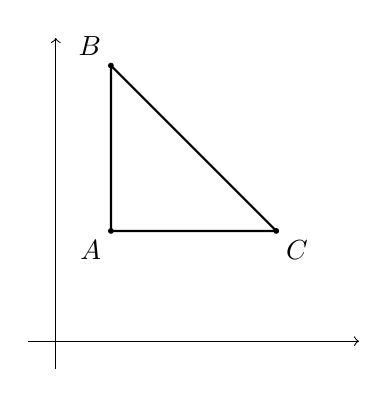
\begin{tikzpicture}[scale=0.7]
  \draw[->] (-0.5,0) -- (5.5,0);
  \draw[->] (0,-0.5) -- (0,5.5);
  \draw[thick] (1,2) -- (1,5) -- (4,2) -- cycle;
  \fill (1,2) circle (1.5pt) node[below left] {\(A\)};
  \fill (1,5) circle (1.5pt) node[above left] {\(B\)};
  \fill (4,2) circle (1.5pt) node[below right] {\(C\)};
\end{tikzpicture}
\end{center}

\textbf{Respuesta final.}
\[
A(1,2),\quad B(1,5),\quad C(4,2),
\qquad
\text{Area}=\frac{9}{2}.
\]
\end{solvedexample}

\begin{commonerror}{Calcular un area antes de tener los vertices}
Si los vertices no estan bien localizados, la base o la altura pueden elegirse mal. En estas
figuras compuestas conviene resolver primero todas las intersecciones necesarias.
\end{commonerror}

\begin{guidedexercise}{[GX-C07.S07-01] Triangulo con los ejes}
Halla los vertices y el area del triangulo delimitado por \(x=0\), \(y=0\) y \(x+y=4\).
\end{guidedexercise}

\begin{shortanswer}{[GX-C07.S07-01]}
Vertices \((0,0)\), \((4,0)\), \((0,4)\). Area \(8\).
\end{shortanswer}

\begin{fullsolution}{[GX-C07.S07-01]}
Los vertices salen de las intersecciones con los ejes:
\[
(0,0),\quad (4,0),\quad (0,4).
\]
El area es
\[
\frac{4\cdot 4}{2}=8.
\]
\end{fullsolution}

\begin{guidedexercise}{[GX-C07.S07-02] Paralelogramo por coordenadas}
Sean \(A(0,0)\), \(B(3,0)\) y \(D(1,2)\). Halla \(C\) y el area del paralelogramo \(ABCD\).
\end{guidedexercise}

\begin{shortanswer}{[GX-C07.S07-02]}
\[
C(4,2),
\qquad
\text{Area}=6.
\]
\end{shortanswer}

\begin{fullsolution}{[GX-C07.S07-02]}
En un paralelogramo, \(C=B+D-A=(4,2)\). La base \(AB\) mide \(3\) y la altura es \(2\), asi que
el area vale \(6\).
\end{fullsolution}

\subsection*{Practica autonoma graduada}
\begin{exercise}{[PX-C07.S07-01] Halla el area del triangulo de vertices \((0,0)\), \((4,0)\) y \((0,3)\).}
\end{exercise}
\begin{exercise}{[PX-C07.S07-02] Halla los vertices y el area del triangulo delimitado por \(x=2\), \(y=1\) y \(x+y=6\).}
\end{exercise}
\begin{exercise}{[PX-C07.S07-03] Sean \(A(1,1)\), \(B(4,1)\) y \(D(2,3)\). Halla \(C\) y el area del paralelogramo \(ABCD\).}
\end{exercise}
\begin{exercise}{[PX-C07.S07-04] Halla los vertices y el area del triangulo delimitado por \(x=0\), \(y=2\) y \(y=x+5\).}
\end{exercise}
\begin{exercise}{[PX-C07.S07-05] Halla el area del triangulo de vertices \((1,1)\), \((5,1)\) y \((3,4)\).}
\end{exercise}
\begin{exercise}{[PX-C07.S07-06] Halla el area del rectangulo delimitado por \(x=0\), \(x=4\), \(y=-1\) y \(y=2\).}
\end{exercise}

\begin{shortanswer}{C07.S07 practica autonoma}
\begin{enumerate}[label=\textbf{PX-C07.S07-\arabic*:}, leftmargin=*]
  \item \(6\)
  \item Vertices \((2,1)\), \((2,4)\), \((5,1)\). Area \(\frac{9}{2}\)
  \item \(C(5,3)\). Area \(6\)
  \item Vertices \((0,2)\), \((0,5)\), \((-3,2)\). Area \(\frac{9}{2}\)
  \item \(6\)
  \item \(12\)
\end{enumerate}
\end{shortanswer}

\begin{fullsolution}{C07.S07 practica autonoma}
\begin{enumerate}[label=\textbf{PX-C07.S07-\arabic*:}, leftmargin=*]
  \item Base \(4\) y altura \(3\): area \(6\).
  \item Las intersecciones son \((2,1)\), \((2,4)\) y \((5,1)\). Base \(3\), altura \(3\).
  \item \(C=B+D-A=(5,3)\). Base \(3\), altura \(2\), area \(6\).
  \item La recta \(y=x+5\) corta a \(x=0\) en \((0,5)\) y a \(y=2\) en \((-3,2)\).
  \item Base \(4\) y altura \(3\): area \(6\).
  \item Lados \(4\) y \(3\): area \(12\).
\end{enumerate}
\end{fullsolution}

\section{[C07.S08] Medianas, alturas y mediatrices}

\subsection*{Objetivos de aprendizaje}
\begin{itemize}
  \item Construir medianas, alturas y mediatrices en coordenadas.
  \item Traducir propiedades geometricas a ecuaciones de rectas.
\end{itemize}

\subsection*{Prerrequisitos}
\begin{itemize}
  \item Puntos medios, pendientes y rectas perpendiculares.
\end{itemize}

\begin{theorybox}{Idea minima}
La mediana une un vertice con el punto medio del lado opuesto. La altura pasa por un vertice y
es perpendicular al lado opuesto. La mediatriz es perpendicular a un segmento y pasa por su
punto medio.
\end{theorybox}

\begin{methodbox}{Como reconocer y resolver}
\begin{enumerate}
  \item Si necesitas una mediana o mediatriz, empieza por hallar un punto medio.
  \item Para una altura, calcula antes la pendiente del lado correspondiente.
  \item Escribe despues la recta con la forma punto-pendiente.
\end{enumerate}
\end{methodbox}

\begin{solvedexample}{[EX-C07.S08-01] Tres rectas notables de un triangulo}
En el triangulo \(A(0,0)\), \(B(6,0)\), \(C(2,4)\), halla:
\begin{itemize}
  \item la mediana trazada desde \(C\);
  \item la altura trazada desde \(C\);
  \item la mediatriz del lado \(AB\).
\end{itemize}

\textbf{Desarrollo.} El punto medio de \(AB\) es
\[
M\left(\frac{0+6}{2},\frac{0+0}{2}\right)=(3,0).
\]
La mediana desde \(C\) pasa por \(C(2,4)\) y \(M(3,0)\). Su pendiente es
\[
\frac{0-4}{3-2}=-4,
\]
asi que
\[
y-4=-4(x-2)
\quad \Longrightarrow \quad
y=-4x+12.
\]
Como \(AB\) es horizontal, la altura desde \(C\) es vertical:
\[
x=2.
\]
La mediatriz de \(AB\) es perpendicular a un segmento horizontal y pasa por \(M\), luego
\[
x=3.
\]

\textbf{Respuesta final.}
\[
\text{Mediana}: y=-4x+12,
\qquad
\text{Altura}: x=2,
\qquad
\text{Mediatriz de } AB: x=3.
\]
\end{solvedexample}

\begin{commonerror}{Usar el vertice en vez del punto medio}
La mediatriz no pasa por un vertice del segmento, sino por su punto medio. Si no se calcula ese
punto primero, la recta sale desplazada.
\end{commonerror}

\begin{guidedexercise}{[GX-C07.S08-01] Mediatriz horizontal}
Halla la mediatriz del segmento con extremos \(A(0,0)\) y \(B(4,0)\).
\end{guidedexercise}

\begin{shortanswer}{[GX-C07.S08-01]}
\[
x=2.
\]
\end{shortanswer}

\begin{fullsolution}{[GX-C07.S08-01]}
El punto medio es \((2,0)\) y el segmento es horizontal, asi que su mediatriz es vertical:
\[
x=2.
\]
\end{fullsolution}

\begin{guidedexercise}{[GX-C07.S08-02] Altura a una horizontal}
Halla la altura trazada desde \(C(1,3)\) al lado \(AB\) de ecuacion \(y=1\).
\end{guidedexercise}

\begin{shortanswer}{[GX-C07.S08-02]}
\[
x=1.
\]
\end{shortanswer}

\begin{fullsolution}{[GX-C07.S08-02]}
Como \(AB\) es horizontal, la altura es vertical y pasa por \(C\), luego \(x=1\).
\end{fullsolution}

\subsection*{Practica autonoma graduada}
\begin{exercise}{[PX-C07.S08-01] Halla el punto medio del segmento con extremos \(A(-1,2)\) y \(B(5,4)\).}
\end{exercise}
\begin{exercise}{[PX-C07.S08-02] Halla la mediatriz del segmento con extremos \(A(2,1)\) y \(B(2,5)\).}
\end{exercise}
\begin{exercise}{[PX-C07.S08-03] Halla la mediana trazada desde \(A(0,0)\) en el triangulo \(A(0,0)\), \(B(4,0)\), \(C(0,2)\).}
\end{exercise}
\begin{exercise}{[PX-C07.S08-04] Halla la altura trazada desde \(A(0,0)\) al lado \(BC\) si \(B(2,0)\) y \(C(2,4)\).}
\end{exercise}
\begin{exercise}{[PX-C07.S08-05] Halla la mediatriz del segmento con extremos \(A(-2,0)\) y \(B(2,0)\).}
\end{exercise}
\begin{exercise}{[PX-C07.S08-06] Halla la mediana trazada desde \(C(0,6)\) en el triangulo \(A(0,0)\), \(B(6,0)\), \(C(0,6)\).}
\end{exercise}

\begin{shortanswer}{C07.S08 practica autonoma}
\begin{enumerate}[label=\textbf{PX-C07.S08-\arabic*:}, leftmargin=*]
  \item \((2,3)\)
  \item \(y=3\)
  \item \(y=\frac{x}{2}\)
  \item \(y=0\)
  \item \(x=0\)
  \item \(y=-2x+6\)
\end{enumerate}
\end{shortanswer}

\begin{fullsolution}{C07.S08 practica autonoma}
\begin{enumerate}[label=\textbf{PX-C07.S08-\arabic*:}, leftmargin=*]
  \item
  \[
  \left(\frac{-1+5}{2},\frac{2+4}{2}\right)=(2,3).
  \]
  \item El segmento es vertical y su punto medio es \((2,3)\), luego la mediatriz es
  horizontal: \(y=3\).
  \item El punto medio de \(BC\) es \((2,1)\). La recta por \((0,0)\) y \((2,1)\) es
  \(y=\frac{x}{2}\).
  \item El lado \(BC\) es vertical, asi que la altura es horizontal: \(y=0\).
  \item El punto medio es el origen y el segmento es horizontal.
  \item El punto medio de \(AB\) es \((3,0)\). La recta por \((0,6)\) y \((3,0)\) es
  \(y=-2x+6\).
\end{enumerate}
\end{fullsolution}

\section{[C07.S09] Bisectrices, ortocentro y lugares geometricos}

\subsection*{Objetivos de aprendizaje}
\begin{itemize}
  \item Hallar bisectrices y ortocentros en casos sencillos.
  \item Interpretar lugares geometricos como ecuaciones de rectas.
\end{itemize}

\subsection*{Prerrequisitos}
\begin{itemize}
  \item Alturas, mediatrices y ecuaciones de rectas.
\end{itemize}

\begin{theorybox}{Idea minima}
Las bisectrices dividen un angulo en dos partes iguales. El ortocentro es el punto de corte de
las alturas de un triangulo. Un lugar geometrico se describe mediante una condicion, por
ejemplo ``todos los puntos equidistantes de dos puntos fijos''.
\end{theorybox}

\begin{methodbox}{Como reconocer y resolver}
\begin{enumerate}
  \item Si el triangulo es rectangulo, el ortocentro coincide con el vertice del angulo recto.
  \item Para puntos equidistantes de dos puntos, piensa en la mediatriz del segmento que los une.
  \item En bisectrices de rectas sencillas, usa simetria y angulos de referencia conocidos.
\end{enumerate}
\end{methodbox}

\begin{solvedexample}{[EX-C07.S09-01] Ortocentro de un triangulo rectangulo}
Halla el ortocentro del triangulo \(A(0,0)\), \(B(4,0)\), \(C(0,3)\).

\textbf{Desarrollo.} Los lados \(AB\) y \(AC\) son perpendiculares, asi que el triangulo es
rectangulo en \(A\). En un triangulo rectangulo, dos alturas coinciden con los propios catetos,
por lo que su punto de corte es el vertice del angulo recto.

\textbf{Respuesta final.}
\[
H=(0,0).
\]
\end{solvedexample}

\begin{commonerror}{Buscar siempre tres alturas completas}
En un triangulo rectangulo no hace falta desarrollar todas las alturas: dos de ellas ya estan
dibujadas en los propios lados.
\end{commonerror}

\begin{guidedexercise}{[GX-C07.S09-01] Bisectrices de los ejes}
Halla las bisectrices de las rectas \(x=0\) e \(y=0\).
\end{guidedexercise}

\begin{shortanswer}{[GX-C07.S09-01]}
\[
y=x
\qquad \text{y} \qquad
y=-x.
\]
\end{shortanswer}

\begin{fullsolution}{[GX-C07.S09-01]}
Los ejes forman cuatro angulos rectos. Sus bisectrices son las diagonales del sistema de ejes:
\[
y=x
\qquad \text{y} \qquad
y=-x.
\]
\end{fullsolution}

\begin{guidedexercise}{[GX-C07.S09-02] Lugar geometrico de equidistancia}
Halla el lugar geometrico de los puntos equidistantes de \(A(-2,0)\) y \(B(2,0)\).
\end{guidedexercise}

\begin{shortanswer}{[GX-C07.S09-02]}
\[
x=0.
\]
\end{shortanswer}

\begin{fullsolution}{[GX-C07.S09-02]}
El lugar geometrico es la mediatriz de \(AB\). Como el segmento es horizontal y su punto medio
es el origen, la mediatriz es
\[
x=0.
\]
\end{fullsolution}

\subsection*{Practica autonoma graduada}
\begin{exercise}{[PX-C07.S09-01] Halla el ortocentro del triangulo \(A(0,0)\), \(B(5,0)\), \(C(0,2)\).}
\end{exercise}
\begin{exercise}{[PX-C07.S09-02] Halla las bisectrices de las rectas \(y=x\) e \(y=-x\).}
\end{exercise}
\begin{exercise}{[PX-C07.S09-03] Halla el lugar geometrico de los puntos equidistantes de \(A(1,1)\) y \(B(5,1)\).}
\end{exercise}
\begin{exercise}{[PX-C07.S09-04] Halla el punto de la recta \(y=2\) que esta a la misma distancia de \(A(0,0)\) y \(B(4,0)\).}
\end{exercise}
\begin{exercise}{[PX-C07.S09-05] Halla el ortocentro del triangulo \(A(1,1)\), \(B(5,1)\), \(C(3,3)\).}
\end{exercise}
\begin{exercise}{[PX-C07.S09-06] Halla el lugar geometrico de los puntos equidistantes de los ejes coordenados en los cuadrantes I y III.}
\end{exercise}

\begin{shortanswer}{C07.S09 practica autonoma}
\begin{enumerate}[label=\textbf{PX-C07.S09-\arabic*:}, leftmargin=*]
  \item \((0,0)\)
  \item \(x=0\) e \(y=0\)
  \item \(x=3\)
  \item \((2,2)\)
  \item \((3,3)\)
  \item \(y=x\)
\end{enumerate}
\end{shortanswer}

\begin{fullsolution}{C07.S09 practica autonoma}
\begin{enumerate}[label=\textbf{PX-C07.S09-\arabic*:}, leftmargin=*]
  \item Es rectangulo en \(A\), luego \(H=A=(0,0)\).
  \item Las rectas dadas son perpendiculares y simetricas respecto de los ejes, que actuan como
  bisectrices.
  \item El segmento \(AB\) es horizontal y su punto medio es \((3,1)\), asi que la mediatriz es
  \(x=3\).
  \item Los puntos equidistantes de \(A\) y \(B\) cumplen \(x=2\). Con \(y=2\), sale \((2,2)\).
  \item Los lados \(AC\) y \(BC\) son perpendiculares, luego el triangulo es rectangulo en \(C\)
  y el ortocentro es \(C=(3,3)\).
  \item La distancia a ambos ejes coincide cuando \(|x|=|y|\). En los cuadrantes I y III eso da
  \(y=x\).
\end{enumerate}
\end{fullsolution}

\section{[C07.S10] Condiciones geometricas combinadas}

\subsection*{Objetivos de aprendizaje}
\begin{itemize}
  \item Resolver problemas que mezclan varias condiciones geometricas.
  \item Detectar cuando un sistema de condiciones no es compatible.
\end{itemize}

\subsection*{Prerrequisitos}
\begin{itemize}
  \item Mediatrices, areas y lugares geometricos.
\end{itemize}

\begin{theorybox}{Idea minima}
Los problemas combinados suelen encadenar lugares geometricos: ``estar a igual distancia'',
``pertenecer a una recta'', ``tener una altura fija'' o ``ser centro de una figura''. La
solucion aparece en la interseccion de esas condiciones, si existe.
\end{theorybox}

\begin{methodbox}{Como reconocer y resolver}
\begin{enumerate}
  \item Traduce cada condicion a una recta, una distancia o un area.
  \item Busca la interseccion de todas las condiciones.
  \item Comprueba al final si esa interseccion existe y tiene sentido geometricamente.
\end{enumerate}
\end{methodbox}

\begin{solvedexample}{[EX-C07.S10-01] Triangulo isosceles con altura fijada}
La base de un triangulo isosceles es el segmento con extremos \(A(-2,0)\) y \(B(2,0)\). El
vertice \(C\) esta sobre la recta \(y=3\). Halla \(C\) y el area del triangulo.

\textbf{Desarrollo.} En un triangulo isosceles con base \(AB\), el vertice \(C\) debe estar en
la mediatriz de \(AB\). Como \(AB\) es horizontal y su punto medio es el origen, la mediatriz es
\[
x=0.
\]
Ademas \(C\) esta en \(y=3\), asi que
\[
C=(0,3).
\]
La base mide \(4\) y la altura es \(3\), luego
\[
\text{Area}=\frac{4\cdot 3}{2}=6.
\]

\textbf{Respuesta final.}
\[
C(0,3),
\qquad
\text{Area}=6.
\]
\end{solvedexample}

\begin{commonerror}{Olvidar una de las condiciones}
Si solo impones que \(C\) este en \(y=3\), hay infinitos candidatos. El rasgo isosceles aporta
otra condicion imprescindible: pertenecer a la mediatriz de la base.
\end{commonerror}

\begin{guidedexercise}{[GX-C07.S10-01] Centro por simetria}
En un hexagono regular, dos vertices opuestos son \(A(-4,0)\) y \(D(4,0)\). Halla el centro.
\end{guidedexercise}

\begin{shortanswer}{[GX-C07.S10-01]}
\[
O(0,0).
\]
\end{shortanswer}

\begin{fullsolution}{[GX-C07.S10-01]}
El centro de un poligono regular es el punto medio de cualquier pareja de vertices opuestos.
Luego
\[
O\left(\frac{-4+4}{2},0\right)=(0,0).
\]
\end{fullsolution}

\begin{guidedexercise}{[GX-C07.S10-02] Equidistancia sobre una recta}
Halla el punto del eje \(X\) equidistante de \(A(-2,2)\) y \(B(2,2)\).
\end{guidedexercise}

\begin{shortanswer}{[GX-C07.S10-02]}
\[
(0,0).
\]
\end{shortanswer}

\begin{fullsolution}{[GX-C07.S10-02]}
Los puntos equidistantes de \(A\) y \(B\) estan en la mediatriz del segmento \(AB\), que es
\(x=0\). Al imponer ademas que el punto este en el eje \(X\), queda \((0,0)\).
\end{fullsolution}

\subsection*{Practica autonoma graduada}
\begin{exercise}{[PX-C07.S10-01] La base de un triangulo isosceles es \(A(0,0)\), \(B(4,0)\) y su vertice esta en la recta \(x=2\) y tiene ordenada \(3\). Halla el vertice y el area.}
\end{exercise}
\begin{exercise}{[PX-C07.S10-02] Halla el punto de la recta \(y=1\) equidistante de \(A(0,0)\) y \(B(4,0)\).}
\end{exercise}
\begin{exercise}{[PX-C07.S10-03] Halla el centro del cuadrado de vertices \((-2,-2)\), \((2,-2)\), \((2,2)\), \((-2,2)\).}
\end{exercise}
\begin{exercise}{[PX-C07.S10-04] La base de un triangulo isosceles es \(A(-3,0)\), \(B(3,0)\) y su altura es \(4\). Halla el area.}
\end{exercise}
\begin{exercise}{[PX-C07.S10-05] En un hexagono regular de centro \(O(0,0)\), un vertice es \(A(2,0)\). Halla el vertice opuesto.}
\end{exercise}
\begin{exercise}{[PX-C07.S10-06] Decide si existe un punto de la recta \(x=1\) equidistante de \(A(0,0)\) y \(B(4,0)\).}
\end{exercise}

\begin{shortanswer}{C07.S10 practica autonoma}
\begin{enumerate}[label=\textbf{PX-C07.S10-\arabic*:}, leftmargin=*]
  \item \(C(2,3)\). Area \(6\)
  \item \((2,1)\)
  \item \((0,0)\)
  \item \(12\)
  \item \((-2,0)\)
  \item No existe
\end{enumerate}
\end{shortanswer}

\begin{fullsolution}{C07.S10 practica autonoma}
\begin{enumerate}[label=\textbf{PX-C07.S10-\arabic*:}, leftmargin=*]
  \item Las condiciones ya fijan \(C=(2,3)\). La base mide \(4\) y la altura \(3\), asi que el
  area es \(6\).
  \item El lugar equidistante de \(A\) y \(B\) es \(x=2\). Con \(y=1\), sale \((2,1)\).
  \item El centro es el punto medio de cualquier diagonal del cuadrado.
  \item Base \(6\) y altura \(4\): area \(12\).
  \item El vertice opuesto al punto \((2,0)\) respecto del centro es \((-2,0)\).
  \item Los puntos equidistantes de \(A\) y \(B\) cumplen \(x=2\). Como eso no corta a la recta
  \(x=1\), no existe solucion.
\end{enumerate}
\end{fullsolution}

\begin{selfcheck}
\begin{itemize}
  \item Distingo cuando conviene trabajar con pendientes, cuando con forma general y cuando con
  puntos medios o mediatrices.
  \item Si dos rectas intervienen en el problema, compruebo antes si son secantes, paralelas o
  coincidentes.
  \item En los lugares geometricos, escribo todas las condiciones antes de resolver.
\end{itemize}
\end{selfcheck}

\begin{extension}{Compatibilidad geometrica}
Un problema puede estar bien planteado algebraicamente y, aun asi, no tener solucion
geometrica. Detectar esas incompatibilidades es parte del razonamiento matematico del bloque,
no un fallo del calculo.
\end{extension}
